\section{Accuracy calculation}\label{accuracy_calculation}


In order to estimate the overfill and underfill, we need to accurately calculate the area covered by a single extrusion path.
If we would simply use an isosceles trapezoidal area, we would get overfill artifacts at corners in the toolpath (\cref{segment_visualization_blocky}).
We therefore use a semi-circle (\cref{segment_visualization_rounded}) with a diameter equal to the starting width in the one end of each segment, and exclude it at the other end, because it will be included in the next segment.
For polyline extrusion paths which are not closed, we also include the semi-circle of the destination location (\cref{segment_visualization_excluded}).

%In order to print such extrusion paths accurately, we can modulate the amount of material flow per millimeter based on this visualization model.
%See \cref{segment_visualization}.

\begin{figure}
\centering
\setlength{\figwidth}{.25\columnwidth}
\begin{subfigure}{\figwidth}\centering
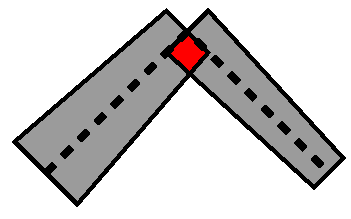
\includegraphics[width=\columnwidth]{sources-validation-visualization-principle-blocky.pdf}
\caption{Blocky}\label{segment_visualization_blocky}
\end{subfigure}
\begin{subfigure}{\figwidth}\centering

\includegraphics[width=\columnwidth]{sources-validation-visualization-principle-rounded.pdf}
\caption{Rounded}\label{segment_visualization_rounded}
\end{subfigure}
\begin{subfigure}{\figwidth}\centering
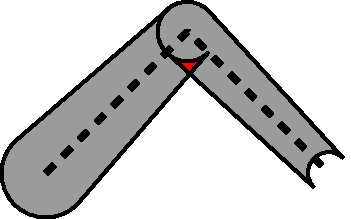
\includegraphics[width=\columnwidth]{sources-validation-visualization-principle-rounded-excluded.pdf}
\caption{Excluded}\label{segment_visualization_excluded}
\end{subfigure}
\caption{
Extruded area of two extrusion segments.
Red areas signify doubly extruded areas.
}
\label{segment_visualization}
\end{figure}

Using boolean operations we can obtain the polygonal regions for overfill and those for underfill.
In order to deal with rounding errors we perform a morphological close of \SI{5}{\micro\meter}, before calculating the total area in \si{\milli\meter\square}.
We also calculate regions which are covered thrice by different extrusion segments and add twice its area to the total overfill area amount.

